\ifpdf
    \graphicspath{{Sections/4_results_figs/Raster/}{Sections/4_results_figs/PDF/}{Sections/4_results_figs/}}
\else
    \graphicspath{{Sections/4_results_figs/Vector/}{Sections/4_results_figs/}}
\fi

\chapter{Additional Figures}
\label{chap:additional-figures}

This appendix contains the extended 20- and 8-view examples and the full patch-size panel. Dataset-size, position and sampler figures are placed with their analyses in the Results section.

\begin{figure}[htbp]
\centering
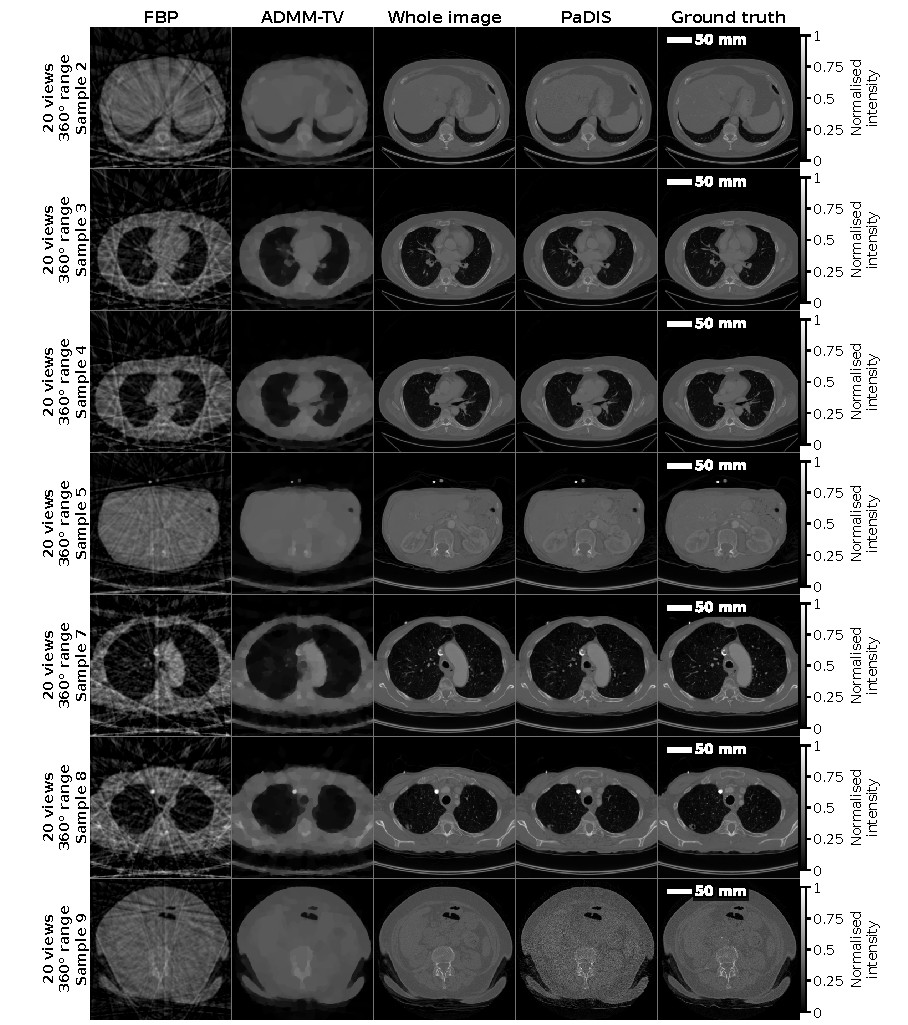
\includegraphics[width=1\textwidth]{figureA1_ct20_additional.pdf}
\caption[Additional 20-view examples.]{Additional 20-view, $360^\circ$ fan-beam examples in NI. Rows are test slices and columns compare FDK, CP, whole-image VE-DPS, PaDIS-VE-DPS and ground truth.}
\label{fig:results-ct20-additional}
\end{figure}

\begin{figure}[htbp]
\centering
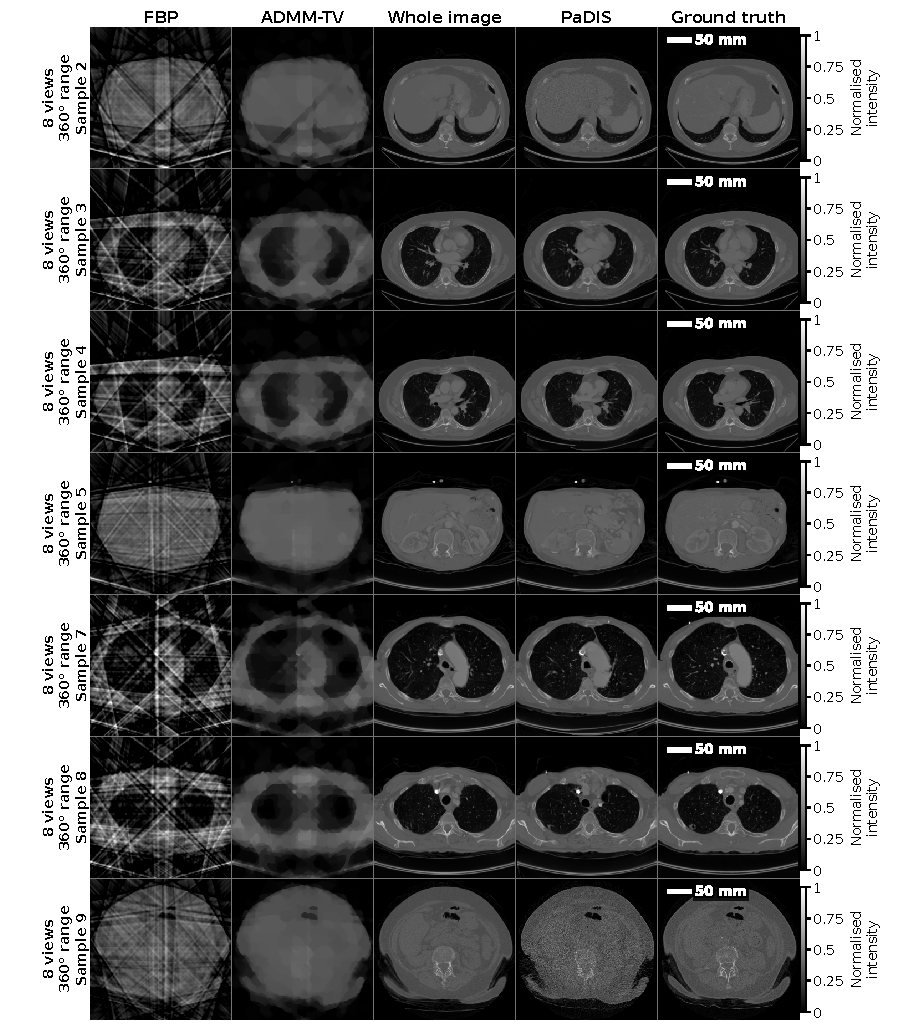
\includegraphics[width=1\textwidth]{figureA2_ct8_additional.pdf}
\caption[Additional 8-view examples.]{Additional 8-view, $360^\circ$ fan-beam examples in NI. Rows are test slices and columns compare FDK, CP, whole-image VE-DPS, PaDIS-VE-DPS and ground truth.}
\label{fig:results-ct8-additional}
\end{figure}

\begin{figure}[htbp]
\centering
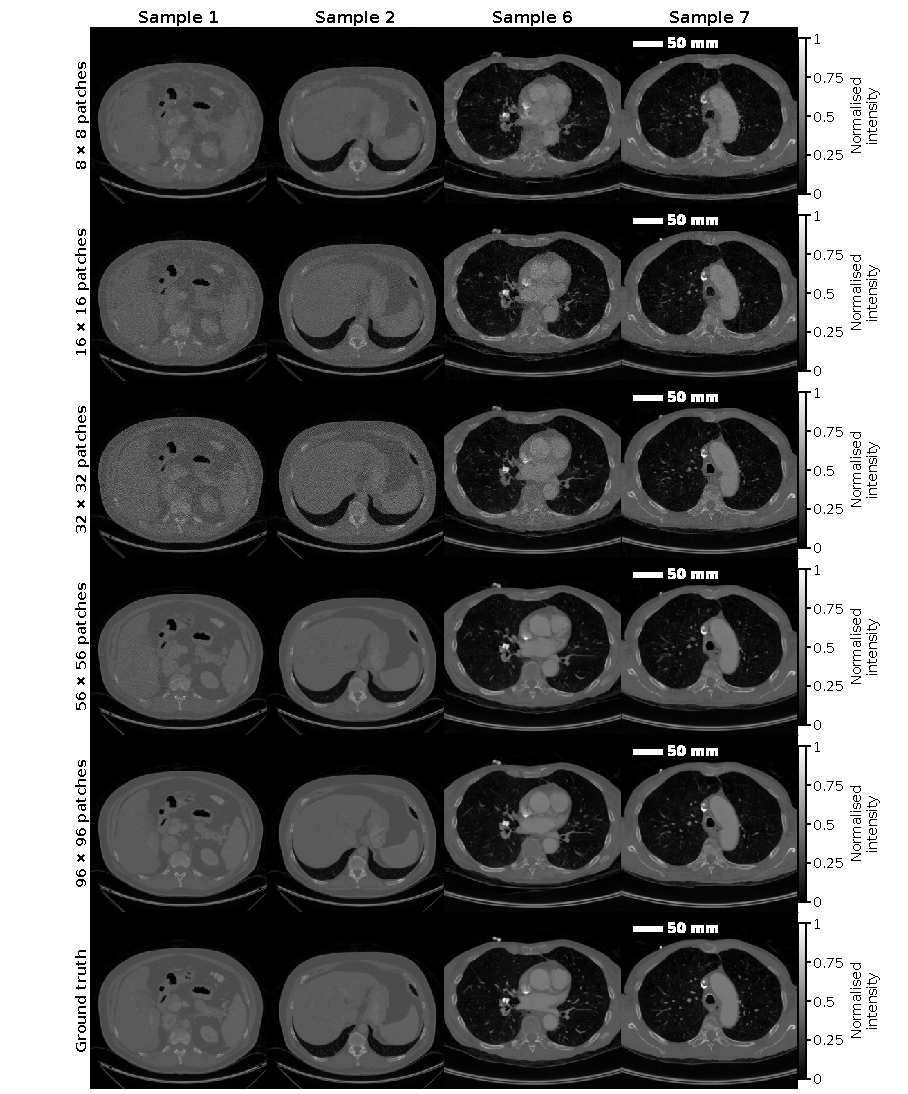
\includegraphics[width=1\textwidth]{figureA5_patch_size.pdf}
\caption[Patch-size reconstruction examples.]{PaDIS-VE-DPS reconstructions from the patch-size ablation in NI. Rows show the maximum training patch size and ground truth. Columns are four test slices. The non-default models inherit the $P=56$ inference setting rather than being tuned separately.}
\label{fig:results-patch-size}
\end{figure}
